\documentclass[
	12pt,			
	openright,		
	oneside,			
	a4paper,		
	english,			
	]{article}
\usepackage[utf8]{inputenc}
\usepackage{graphicx,float}
\usepackage{blindtext}
%\usepackage[belowskip=-15pt,aboveskip=0pt]{caption}
\usepackage[colorlinks=true, linkcolor=blue]{hyperref}
\hypersetup{
    colorlinks=true,
    linkcolor=blue,
    filecolor=magenta,      
    urlcolor=cyan,
}
\usepackage{multicol}


%\setlength\parindent{1cm}



\begin{document}

\begin{titlepage}


\vspace*{-1in}
\begin{figure}[htb]
\centering

\includegraphics[width=2.5cm]{Slike/logo.png}

\end{figure}
\begin{center}
\begin{large}    {Univerzitet u Beogradu, Matematički fakultet \\
    }
    \end{large}
    \vspace*{0.2in}
    \begin{large}    {Istraživanje podataka 1 
    }
    \end{large}

\end{center}

        \vspace*{1.8in}


        \begin{center}
            
       \vspace*{0.2in}
        \begin{huge}
        \textbf{Oružano nasilje u SAD \\
               seminarski rad}
        \\
        \end{huge}
        \vspace*{2in}
         \end{center}
        
        \begin{large}{\noindent
        autor: Luka Banović, 80/2016 
        \\   profesor: Nenad Mitić
        \\   asistent: Mirjana Maljković
        }
        \end{large}
        \vspace*{0.5in}
        
        \centering
        \begin{large}{
        Jun 2019}
        \end{large}
        
        
        \end{titlepage}

\tableofcontents
\newpage

\section{Uvod}

Ovaj rad obradjuje skup podataka oružanog nasilja u Sjedinjenim \\ Američkim Državama, koji sadrži podatke od početka 2013. godine,\\ do 3. meseca 2018. godine.
Skup podataka se nalazi na linku: \\ \url{https://www.kaggle.com/jameslko/gun-violence-data}\\
Metoda kojom se obradjuju podaci je klasterovanje, korišćenjem \\
različitih algoritama.



\subsection{Motivacija}
Skup podataka mi je izgledao interesantno sa aspekta mogućnosti \\
izvlačenja korisnih zaključaka koji su primenljivi u praksi, \\
bilo da je u pitanju izvlačenje zakonitosti u odnosu na oblasti, \\
predvidjanje budućih incidenata na osnovu nekih drugih zakonitosti \\
i slično.

\subsection{Cilj}
Ideja je bila da sa završetkom rada budu izvedena neka pravila,\\ zakonitosti ili korisne informacije o povezanosti odredjenih\\
faktora navedenih u podacima. Medjutim, sa obzirom na veliku  \\
količinu podataka i svoje neiskustvo u radu sa njima, uspeo \\ 
sam samo da analiziram podatke i izvedem svoje zaključke \\
koji mogu biti korisni, a i ne moraju.

\subsection{Struktura rada}
Rad je podeljen u više oblasti, redosledom kojim su sprovodjeni \\
postupci. Objašnjeno je, redom, upoznavanje sa podacima, \\
pretprocesiranje, algoritmi klasterovanja i zaključak rada.

\newpage
\section{Upoznavanje sa podacima}
Skup podataka sadrži 29 atributa i 239677 redova. \\
Deo atributa neće biti korišćen u algoritmima, ali će ovde biti navedeni svi.
\begin{multicols}{2}
\begin{itemize}
    \item {incident\_id: jedinstveni broj incidenta}
    \item date: datum incidenta
    \item state: savezna država 
    \item city\_or\_county: grad ili okrug
    \item address: adresa na kojoj se dogodio incident
    \item n\_killed: broj ubijenih ljudi
    \item n\_injured: broj povredjenih ljudi
    \item incident\_url: URL informacije o incidentu
    \item source\_url: referenca ka reportaži o incidentu
    \item incident\_url\_fields\_missing: da li nedostaje podatakak icident\_url
    \item congressional\_district: Jedinstveni broj kongresnog distrikta
    \item gun\_stolen: da li je oružije ukradeno
    \item gun\_type: tip oružja
    \item incident\_characteristics: karakteristike incidenta
    \item latitude: geografska širina
    \item longitude: geografska dužina
    \item location\_description: opis lokacije
    \item n\_of\_guns\_involved: broj oružija koje je učestvovalo
    \item notes: dodatne informacije 
    \item participant\_age: godine učesnika u vreme incidenta
    \item participant\_age\_group: Starosna grupa učesnika
    \item participant\_gender: Pol učesnika
    \item participant\_name: ime učesnika
    \item participant\_relationship: bračni status učesnika
    \item participant\_type: tip učesnika - žrtva, počinilac
    \item sources: izvor o učesnicima
    \item state\_house\_district: izborna ćelija distrikta
    \item state\_senate\_district: teritorija izborne ćelije za senat
\end{itemize}
\end{multicols}

\newpage
\section{Pretprocesiranje podataka}



Pretprocesiranje je radjeno u IBM SPSS Modeleru. \\
Odbačeno je preko 50\% atributa, iz različitih razloga. \\
Veliki deo je odbačen iz razloga što imaju ogroman broj \\
različitih vrednosti. \\
Takodje su izbačeni atributi sa
jedinstvenim vrednostima iz razloga\\
što algoritmi klasterovanja
grupišu podatke na osnovu sličnosti. \\

Zatim su, zbog prevelikog broja nedostajućih vrednosti \\
odnosno praznina izbačeni atributi gun\_tupe, participant\_age, \\
i num\_of\_guns\_involved.\\

Sledeći korak je bio pretvaranje polja date u tri različita: \\
\begin{itemize}
    \item Year (2013-2018)
    \item Month (1-12)
    \item Day (1-7)
\end{itemize}{}
koji imaju numeričke vrednosti, radi lakše obrade. \\

Poslednje uradjeno je računanje num\_of\_participants, \\
atribut u kom smo sačuvali broj učesnika.

Na kraju, podaci s kojima je radjeno su izgledali ovako: \\




    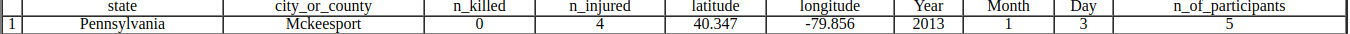
\includegraphics[width = 15cm]{Slike/final.png}

\newpage
\section{Klasterovanje}
Klasterovanje je tehnika istraživanja podataka koja otkriva objekte \\ podataka sličnih osobina i deli ih u grupe (klastere), čineći ih \\ preglednijim i korisnijim. \\
U ovom radu primenjeni su različiti algoritmi, opisani u narednim \\
sekcijama.

\subsection{K-Means algoritam}
    Pri radu sa algoritmom k-sredina bilo mi je smisleno da 
    podelim\\ u 4 segmenta. Prvi je uzimao u obzir sve atribute 
    sem meseca i dana\\ - dakle grupisao je po godinama. Shodno tome,  drugi je uzimao sve\\ atribute sem meseca, a treći sve atribute  sem dana u nedelji. Četvrta verzija uzimala je u obzir sve
    atribute, i postigla najlošije rezultate. \\
    Za svaki segment rad je izgledao ovako: \\
    Algoritam je podešavan da proizvede od 5 do 15 klastera sa  korakom 1, \\a zatim do 50 sa korakom 5.
    
    \subsubsection{K-Means, Year}
    Najbolji rezultati u smislu prosečnog koeficijenta senke dobijeni  su za varijante 5 i 20 klastera.
    Raspored instanci po klasteru izgleda ovako: 
    \begin{center}
    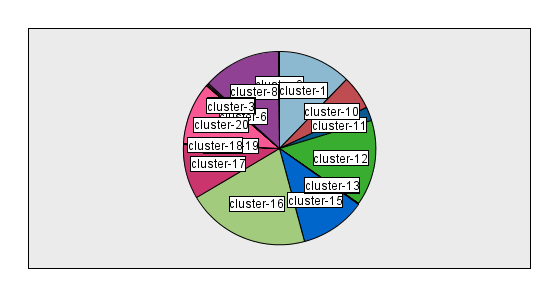
\includegraphics[width = 15cm]{Slike/KMeans_Year20.png}
    \end{center}
    
    Zaključak - algoritam je koristio sve atribute sa jednakom važnosti, te se najveća razlika vidi u godinama incidenata.
    Dva od 5 klastera imaju 2016. godinu, a oni se izmedju sebe
    razlikuju po broju učesnika, gde prvi klaster ima prosečan broj
    povredjenih i smrti mnogo veći od drugog. Nakon godine incidenta, klasteri se medjusobno razlikuju i po lokaciji(geografskoj širini i dužini) dok su po prosečnom broju povredjenih i žrtava slični.
    

    Što se tiče verzije sa 20 klastera, raspored instanci po klasterima je bio bolji, dok je koeficijent senke bio za nijansu manji od prethodnog.
    Klasteri su bili slični po broju učesnika, dok su se najviše razlikovali po broju umrlih i broju povredjenih, pa zatim i po lokaciji.
    \\
    Raspored instanci je izgledao ovako:
    \begin{center}
    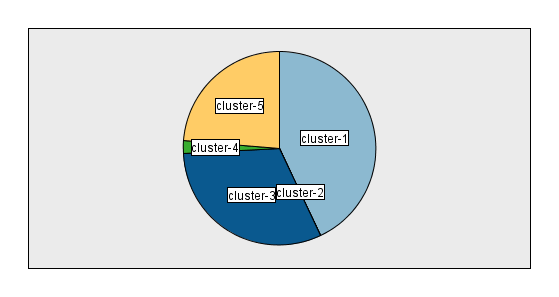
\includegraphics[width = 15cm]{Slike/KM_Year5.png}
    \end{center}
    \subsubsection{K-Means, Month}
    Za verziju koja je uzimala u obzir polje Month, najbolje koeficijente senke postigle su opcije sa 6 i 12 klastera.
    Kod varijante sa 6 klastera, razlike su po mesecima, lokacini i broju smrti, dok su slični po broju učesnika, i broju ubijenih.
    \newpage
    Nakon koriščenja PCA/Factor čvora u SPSS Modeleru, raspored klastera izgleda ovako: 
    \begin{center}
    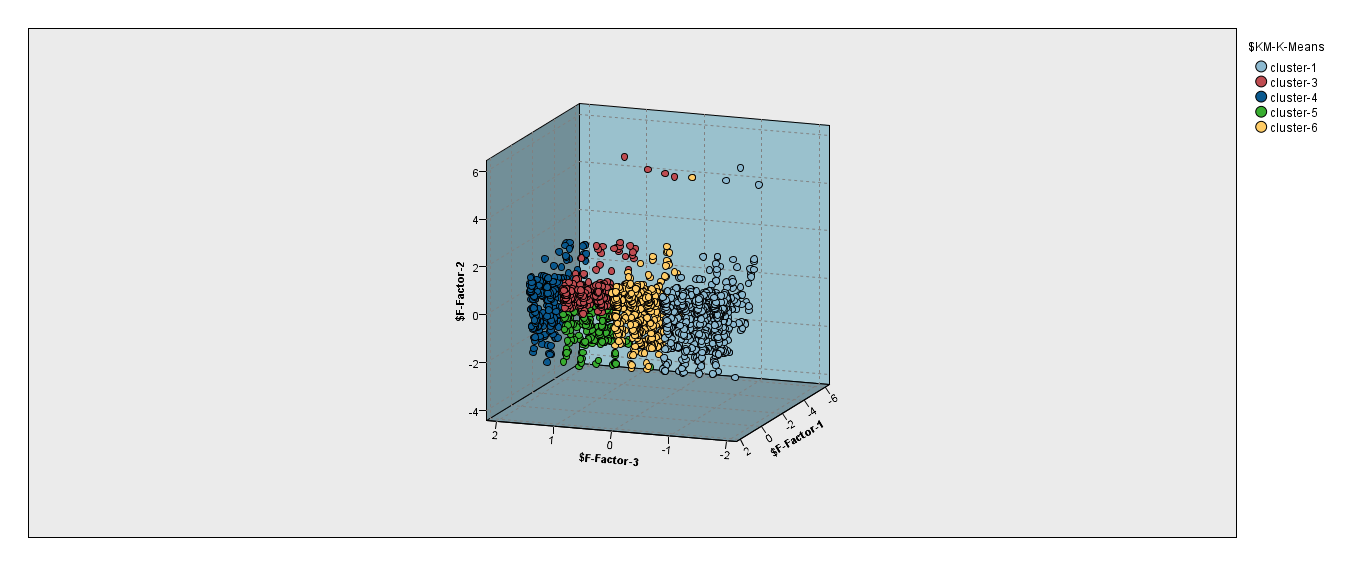
\includegraphics[width = 15cm]{Slike/KM_Month6.png}
    \end{center}
    Verzija sa 12 klastera, raspored instanci po klasterima izgleda ovako: 
    \begin{center}
    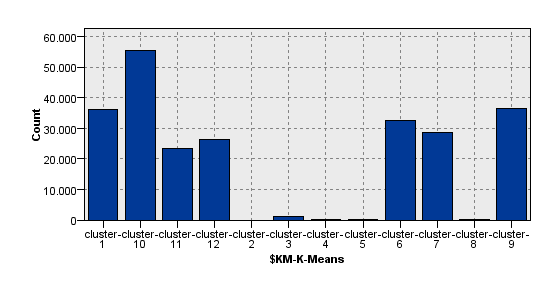
\includegraphics[width = 15cm]{Slike/KMMonth12.png}
    \end{center}
    Atribut Month je onaj po kome se klasteri najviše razlikuju, a zatim lokacija. Slični su po broju povredjenih, broju smrti i broju učesnika, osim par klastera u koje su svrstani ekstremni slučajevi.
    \newpage
    
    \subsubsection{K-Means, Day}
    Ovde je algoritam dao najbolje rezultate za verzije sa 6 i 7 klastera. \\
    U obe verzije se klasteri najvise razlikuju po atributu Day, gde se specijalno izdvajaju 2 klastera sa ekstremnim vrednostima broja učesnika.
    Takodje, jedan klaster sa malim brojem instanci se isticao po lokaciji, imajući geografsku širinu i dužinu dosta različitu od ostalih. Uz malo istraživanja gde se to nalazi sam zaključio da se u oblasti krajnjeg severozapada Sjedinjenih Američkih Država  desilo u proseku znatno manje incidenata u odnosu na ostale teritorije.\\
    Prosečan broj učesnika, poginulih i ranjenih je veoma sličan kod svih klastera, te možemo zaključiti da se, na osnovu rezultata za dane, najviše incidenata dogodilo subotom i nedeljom, a zatim neznatno manje ponedeljkom.
    
    \begin{center}
    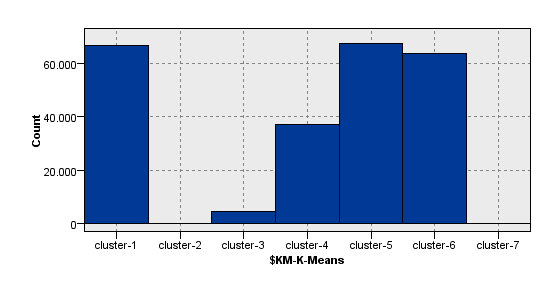
\includegraphics[width = 15cm]{Slike/KMDay7.png}
    \end{center}
    
    Verzija koja je uzimala u obzir sve atribute je imala veoma loš koeficijent senke za svaku od iteracija sa različitim klasterima.
    Koeficijent senke se nije menjao kroz iteracije, te je bilo koja reprezentativna. Nisam uspeo da izvučem nikakve smislene zaključke te neću obradjivati tu verziju ovde.
\newpage
\subsection{Kohonen}
U radu sa Kohonen algoritmom još jednom sam naišao na to da uzimanjem u obzir svih podataka algoritam ne daje smislene rezultate. Pri svakoj iteraciji algoritam je davao broj klastera jednak maksimalnom dozvoljenom, uz loš koeficijent senke, te sam ponovo podelio na više verzija, iterativno ograničavajući broj klastera.
Jedine solidne koeficijente senke imale su opcije koje uzimaju u obzir godinu i mesec.\\
Verzija koje uzima u obzir atribut Year je imala 3 klastera, raspored instanci je izgledao ovako: 
 \begin{center}
    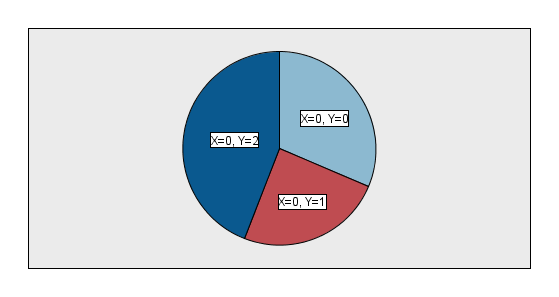
\includegraphics[width = 15cm]{Slike/KohonenYear.png}
    \end{center}

Ovde je važnost ulaznih vrednosti vila visoka jedino za polje Year, dok je za ostale bila značajno manja.

\newpage
Verzija koja uzima atribut Month, imala je 15 klastera, dok je raspored instanci po klasterima izgledao ovako:


 \begin{center}
    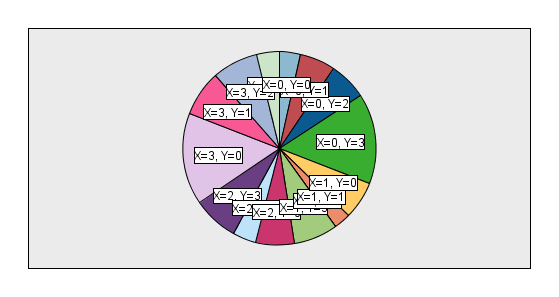
\includegraphics[width = 15cm]{Slike/KohonenMonth.png}
    \end{center}

U ovoj varijanti, značaj ulaznih vrednosti(prediktora) je bila podjednaka za sve atribute te su rezultati bili bolji.
        
\subsection{Hijerarhijsko klasterovanje}
Hijerarhijsko klasterovanje mi je bilo posebno problematično. 
Zbog dimenzionalnosti nisam mogao adekvatno da izvršim algoritme hijerarhijskog klasterovanja kao i DBScan, medjutim kod hijerarhijskog klasterovanja sam imao više problema.
Zbog izbacivanja greške koja signalizira nedostatak memorije, uzeo sam uzorak od 10000 redova, da bi uopšte algoritam mogao da radi. Medjutim, cilj da se dobiju iole smisleni rezultati nije uspeo, te ni vizuelizacija nije uspela.
Rezultat - 2 klastera.

\subsection{DBSCAN algoritam}
DBScan algoritam je takodje imao problema sa dimenzionalnosti, te je zahtevao veoma mnogo vremena za izvršavanje.
U pokušaju da osposobim algoritam, podesio sam parametar min\_samples na 2 i uspeo. Rezultat - 13 klastera, koeficijent senke oko 0,49.
Bez obzira na broj klastera, raspored nije bio dobar, dva klastera su saržala skoro 99\% svih instanci.
Kao ni u prethodom algoritmu, nisam uspeo da zaključim ništa korisno 




\section{Zaključak}
Proces izrade ovog rada je definitivno bio zanimljiv, iako ne toliko uspešan. Svakako sam veoma mnogo naučio kroz mnogo neuspelih pokušaja.
Ciljevi sa početka su delimično ostvareni, u smislu da sam uspeo izvući par zaključaka, medjutim da li su oni korisni za neku praktičnu primenu nisam siguran. 
\\
Ono u šta sam siguran jeste da se, uz ekstenzivniju i kompetentniju analizu ovog skupa podataka zaista može doći do korisnih zaključaka, koji će možda i omogućiti predvidjanje i prevenciju budućih incidenata, a ako ne to, onda samo upozorenja u oblastima i periodima veće učestalosti krivičnih dela.


        
        
\end{document}

